\documentclass[tikz,border=2pt]{standalone}
\usepackage{tikz}
\usetikzlibrary{positioning}
\begin{document}
	\begin{tikzpicture}[
	main/.style={rectangle, rounded corners, text centered, text width=3cm, draw=black},
	aux/.style={}
	]	
	
	\node (project) [main] {Project};
	
		\node (results) [main, below=of project] {Results and conclusions};
		
		\node (sim) [main, left=4cm of results] {Simulation};
			\node (aux2) [aux, below=of sim] {};
			\node (mathsim) [main, left=1.5cm of aux2] {Mathematical Simulation};
			\node (visualsim) [main, right=1.5cm of aux2] {Visual simulation};
				\node (aux6) [aux, below=of visualsim] {};
				\node (simulatequad) [main, left=of aux6] {Simulate quad};
				\node (simulateenvironm) [main, right=of aux6] {Simulate environment \& obstacles};
		
		\node (mod) [main, left=17cm of sim] {Modelling};
			\node (controlandblock) [main, below=of mod] {Control Theory/ Block Diagram};
				\node (aux4) [aux, below=of controlandblock] {};
				\node (statemodel) [main, left=of aux4] {State model equation};
				\node (blockdiagram) [main, right=of aux4] {Block diagram};
			\node (mathmodel) [main, left=8cm of controlandblock] {Mathematical modelling of quad \& sensors};
				\node (dynamics) [main, below=of mathmodel] {Dynamics};	
				\node (kinematics) [main, left=of dynamics] {Kinematics};
				\node (sensorsmodels) [main, right=of dynamics] {Sensors models};
			\node (quadtrack) [main, right=6cm of controlandblock] {Quad tracking};
				\node (aux5) [aux, below=of quadtrack] {};
				\node (potfields) [main, left=of aux5] {Potential fields};
				\node (astar) [main, right=of aux5] {A* and others};
			
		
		\node (lit) [main, left=23cm of mod] {Literature};
			\node (aux1) [aux, below=of lit] {};
			\node (matsimlit) [main, left=of aux1] {MatLab Simulation};
				\node (mathworks) [main, below=of matsimlit] {Search Google \& MathWorks};
			\node (modlit) [main, left=3cm of matsimlit] {Quads modelling};
				\node (aux3) [aux, below=of modlit] {};
				\node(weighandforces)[main, left=of aux3] {Quad weight \& forces model in IEEE journals};
				\node(movement)[main, right=of aux3] {Quad movement model in IEEE journals};
			\node (sensorslit) [main, right=of aux1] {Sensors};
				\node (sensorsjour) [main, below=of sensorslit] {Model \& use of sensors in drones in IEEE journals};
			\node (trackinglit) [main, right=of sensorslit] {Tracking};
				\node (trackjour) [main, below=of trackinglit] {Read articles in IEEE journals};
			
		\node (rep) [main, right=of results] {Report};
		\node (peerrev) [main, right=of rep] {Peer-Review};	

	\draw [-latex] (project.south)--++(0,-.3)-| (lit.north);
	\draw [-latex] (project.south)--++(0,-.3)-| (mod.north);
	\draw [-latex] (project.south)--++(0,-.3)-| (sim.north);
	\draw [-latex] (project.south)--++(0,-.3)-| (results.north);
	\draw [-latex] (project.south)--++(0,-.3)-| (rep.north);
	\draw [-latex] (project.south)--++(0,-.3)-| (peerrev.north);
	
	\draw [-latex] (lit.south)--++(0,-.3)-| (matsimlit.north);
	\draw [-latex] (lit.south)--++(0,-.3)-| (modlit.north);
	\draw [-latex] (lit.south)--++(0,-.3)-| (sensorslit.north);
	\draw [-latex] (lit.south)--++(0,-.3)-| (trackinglit.north);
	
	\draw [-latex] (mod.south)--++(0,-.3)-| (controlandblock.north);
	\draw [-latex] (mod.south)--++(0,-.3)-| (mathmodel.north);
	\draw [-latex] (mod.south)--++(0,-.3)-| (quadtrack.north);
	
	\draw [-latex] (sim.south)--++(0,-.3)-| (mathsim.north);
	\draw [-latex] (sim.south)--++(0,-.3)-| (visualsim.north);
		
	\draw [-latex] (matsimlit.south)--++(0,-.3)-| (mathworks.north);
	\draw [-latex] (modlit.south)--++(0,-.3)-| (weighandforces.north);	
	\draw [-latex] (modlit.south)--++(0,-.3)-| (movement.north);
	\draw [-latex] (sensorslit.south)--++(0,-.3)-| (sensorsjour.north);	
	\draw [-latex] (trackinglit.south)--++(0,-.3)-| (trackjour.north);	
	
	\draw [-latex] (controlandblock.south)--++(0,-.3)-| (statemodel.north);	
	\draw [-latex] (controlandblock.south)--++(0,-.3)-| (blockdiagram.north);	
	\draw [-latex] (mathmodel.south)--++(0,-.3)-| (kinematics.north);	
	\draw [-latex] (mathmodel.south)--++(0,-.3)-| (dynamics.north);	
	\draw [-latex] (mathmodel.south)--++(0,-.3)-| (sensorsmodels.north);	
	\draw [-latex] (quadtrack.south)--++(0,-.3)-| (potfields.north);	
	\draw [-latex] (quadtrack.south)--++(0,-.3)-| (astar.north);	
	
	\draw [-latex] (visualsim.south)--++(0,-.3)-| (simulatequad.north);	
	\draw [-latex] (visualsim.south)--++(0,-.3)-| (simulateenvironm.north);	
	
	\end{tikzpicture}
\end{document}